\documentclass[bachelor, och, labwork]{shiza}
% параметр - тип обучения - одно из значений:
%    spec     - специальность
%    bachelor - бакалавриат (по умолчанию)
%    master   - магистратура
% параметр - форма обучения - одно из значений:
%    och   - очное (по умолчанию)
%    zaoch - заочное
% параметр - тип работы - одно из значений:
%    referat    - реферат
%    coursework - курсовая работа (по умолчанию)
%    diploma    - дипломная работа
%    pract      - отчет по практике
% параметр - включение шрифта
%    times    - включение шрифта Times New Roman (если установлен)
%               по умолчанию выключен
\usepackage{subfigure}
\usepackage{tikz,pgfplots}
\pgfplotsset{compat=1.5}
\usepackage{float}

%\usepackage{titlesec}
\setcounter{secnumdepth}{4}
%\titleformat{\paragraph}
%{\normalfont\normalsize}{\theparagraph}{1em}{}
%\titlespacing*{\paragraph}
%{35.5pt}{3.25ex plus 1ex minus .2ex}{1.5ex plus .2ex}

\titleformat{\paragraph}[block]
{\hspace{1.25cm}\normalfont}
{\theparagraph}{1ex}{}
\titlespacing{\paragraph}
{0cm}{2ex plus 1ex minus .2ex}{.4ex plus.2ex}

% --------------------------------------------------------------------------%


\usepackage[T2A]{fontenc}
\usepackage[utf8]{inputenc}
\usepackage{graphicx}
\graphicspath{ {./images/} }
\usepackage{tempora}

\usepackage[sort,compress]{cite}
\usepackage{amsmath}
\usepackage{amssymb}
\usepackage{amsthm}
\usepackage{fancyvrb}
\usepackage{listings}
\usepackage{listingsutf8}
\usepackage{longtable}
\usepackage{array}
\usepackage[english,russian]{babel}

\usepackage[colorlinks=false]{hyperref}
\usepackage{url}

\usepackage{underscore}
\usepackage{setspace}
\usepackage{indentfirst} 
\usepackage{mathtools}
\usepackage{amsfonts}
\usepackage{enumitem}
\usepackage{tikz}
\usepackage{minted}

\newcommand{\eqdef}{\stackrel {\rm def}{=}}
\newcommand{\specialcell}[2][c]{%
\begin{tabular}[#1]{@{}c@{}}#2\end{tabular}}

\renewcommand\theFancyVerbLine{\small\arabic{FancyVerbLine}}

\newtheorem{lem}{Лемма}

\begin{document}

% Кафедра (в родительном падеже)
\chair{теоретических основ компьютерной безопасности и криптографии}

% Тема работы
\title{Арифметические операции в числовых полях}

% Курс
\course{5}

% Группа
\group{531}

% Факультет (в родительном падеже) (по умолчанию "факультета КНиИТ")
\department{факультета КНиИТ}

% Специальность/направление код - наименование
%\napravlenie{09.03.04 "--- Программная инженерия}
%\napravlenie{010500 "--- Математическое обеспечение и администрирование информационных систем}
%\napravlenie{230100 "--- Информатика и вычислительная техника}
%\napravlenie{231000 "--- Программная инженерия}
\napravlenie{100501 "--- Компьютерная безопасность}

% Для студентки. Для работы студента следующая команда не нужна.
% \studenttitle{Студентки}

% Фамилия, имя, отчество в родительном падеже
\author{Улитина Ивана Владимировича}

% Заведующий кафедрой
% \chtitle{} % степень, звание
% \chname{}

%Научный руководитель (для реферата преподаватель проверяющий работу)
\satitle{профессор} %должность, степень, звание
\saname{В. А. Молчанов}

% Руководитель практики от организации (только для практики,
% для остальных типов работ не используется)
% \patitle{к.ф.-м.н.}
% \paname{С.~В.~Миронов}

% Семестр (только для практики, для остальных
% типов работ не используется)
%\term{8}

% Наименование практики (только для практики, для остальных
% типов работ не используется)
%\practtype{преддипломная}

% Продолжительность практики (количество недель) (только для практики,
% для остальных типов работ не используется)
%\duration{4}

% Даты начала и окончания практики (только для практики, для остальных
% типов работ не используется)
%\practStart{30.04.2019}
%\practFinish{27.05.2019}

% Год выполнения отчета
\date{2023}

\maketitle

% Включение нумерации рисунков, формул и таблиц по разделам
% (по умолчанию - нумерация сквозная)
% (допускается оба вида нумерации)
% \secNumbering

%-------------------------------------------------------------------------------------------

\section{Постановка задачи}

    \textbf{Цель работы} - изучение основных операций в числовых полях и их
    программная реализация. 

    Порядок выполнения работы:
    \begin{enumerate}
        \item Разобрать обычный, бинарный и расширенный алгоритмы Евклида
        вычисления наибольшего общего делителя целых чисел и привести их
        программную реализацию;
        \item Разобрать алгоритмы решения систем сравнений и привести их
        программную реализацию;
        \item Рассмотреть метод Гаусса решения систем линейных уравнений над
        конечными полями и привести его программную реализацию.
    \end{enumerate}

\section{Теоретические сведения}

    \subsection{Алгоритм Евклида}

        \textbf{Алгоритм Евклида} вычисления наибольшего общего делителя целых
        чисел $a$ и $b
        > 0$ состоит из следующих этапов. Положим $a_0 = a$, $a_1 = b$ и выполним
        последовательно деления с остатком $a_i$ на $a_{i + 1}$:

        $$a_0 = a_1q_1 + a_2, 0 \leq a_2 < a_1,$$
        $$a_1 = a_2q_2 + a_3, 0 \leq a_3 < a_2,$$
        $$\cdots$$
        $$a_{k - 2} = a_{k - 1}q_{k - 1} + a_k, 0 \leq a_k < a_{k - 1},$$
        $$a_{k - 1} = a_k q_k.$$

        Так как остатки выполняемых делений образуют строго убывающую
        последовательность $a_1 > a_2 > a_3 > \cdots \geq 0$, то этот процесс
        обязательно остановится в результате получения нулевого остатка деления.
        Легко видеть, что НОД($a_0, a_1$) = НОД($a_1, a_2$) = $\cdots$ =
        НОД($a_{k-1}, a_k$) = $a_k$. Значит, последний ненулевой остаток $a_k$ =
        НОД($a,b$).

    \subsection{Расширенный алгоритм Евклида}

        \textbf{Расширенный алгоритм Евклида} позволяет не только вычислять
        наибольший общий делитель целых чисел $a$ и $b > 0$, но и представлять
        его в виде НОД$(a, b)= ax+by$ для некоторых $x, y \in Z$. Значения $x,y$
        находятся в результате обратного прохода этапов алгоритма Евклида, в
        каждом из которых уравнение разрешается относительно остатка $a_i$,
        который представляется в форме $a_i = ax_i + by_i$ для некоторых $x_i,
        y_i \in Z$. В результате получается следующая последовательность
        вычислений:

        $$a_0 = a, a_0 = ax_0 + by_0,$$
        $$a_1 = b, a_0 = ax_1 + by_1,$$
        $$a_2 = a_0 - a_1q_1, a_2 = ax_2 + by_2,$$
        $$a_3 = a_1 - a_2q_2, a_3 = ax_3 + by_3,$$
        $$ \cdots $$
        $$a_i = a_{i - 2} - a_{i - 1}q_{i - 1}, a_i = ax_i + by_i,$$
        $$ \cdots $$
        $$a_k = a_{k - 2} - a_{k - 1}q_{k - 1}, a_k = ax_k + by_k,$$
        $$0 = a_{k - 1} - a_k q_k, 0 = ax_{k + 1} + by_{k + 1}$$

        В правом столбце все элементы $a_k, a_{k-1}, a_{k-2}, . . . , a_1, a_0$
        представляются в виде $a_i = ax_i + by_i$. Очевидно, что $x_0 = 1, y_0 =
        0, x_1 = 0, y_1 = 1$ и выполняются равенства: $a_i = a_{i-2} - a_{i-1}
        q_{i-1}, x_i = x_{i-2} - x_{i-1} q_{i-1}, y_i = y_{i-2} - y_{i-1}
        q_{i-1}$. Отсюда последовательно получаются искомые представления всех
        элементов $a_k, a_{k-1}, a_{k-2}, \dots, a_1, a_0$ и, в частности,
        представление НОД$(a,b) = a_k = ax_k +by_k$.

    \subsection{Бинарный алгоритм Евклида}

        \textbf{Бинарный алгоритм Евклида} является одним из эффективных методов
        нахождения НОД. Пусть даны целые числа $a > b > 0$. Вычисляется
        последовательность упорядоченных пар $(x_k, y_k)$ неотрицательных чисел,
        где $(x_1, y_1) = (a, b)$, и если уже вычислена пара $(x_i , y_i)$, то:

        \begin{enumerate}
            \item находится число $e$ со свойством $2^e y_i \leq x_i \leq
            2^{e+1}y_i$;
            \item вычисляется $t = \min\{2^{e+1} y_i - x_i, x_i - 2^e y_i\} \geq
            0$;
            \item если при этом $t \geq y_i$, то тогда полагаем $(x_{i + 1},
            y_{i + 1}) = (y_i, t)$, а если $t > y_i,$ то полагаем $(x_{i + 1},
            y_{i + 1}) = (t, y_i)$.
        \end{enumerate}
        
        Алгоритм заканчивает свою работу, как только очередное значение
        $y_m$ оказывается равным нулю. При этом наибольшим общим делителем
        чисел $a$ и $b$ является число $x_m$.

        Сам по себе бинарный алгоритм Евклида основан на следующих свойствах:

        \begin{enumerate}
            \item НОД($2 \cdot a, 2 \cdot b$) = $2 \cdot$ НОД($a, b$);
            \item НОД($2 \cdot a, 2 \cdot b + 1$) = НОД($a, 2 \cdot b + 1$)
            \item НОД($-a, b$) = НОД($a, b$).
        \end{enumerate}


    \subsection{Греко-китайская теорема об остатках}

        \textbf{Теорема.} Пусть $m_1, m_2, \dots , m_k$ – попарно взаимно
        простые целые числа и $M = m_1m_2 \cdots m_k$. Тогда система линейных
        сравнений


        \begin{equation}
            \begin{cases}
                x \equiv a_1 (mod \text{ } m_1)\\
                x \equiv a_2 (mod \text{ } m_2)\\
                x \equiv a_3 (mod \text{ } m_3)\\
                \cdots\\
                x \equiv a_k (mod \text{ } m_k)\\              
            \end{cases}\,.
        \end{equation}
        
        имеет единственное неотрицательное решение по модулю $M$. При этом, если
        для каждого $1 \leq j \leq n$ число $\frac{M}{m_j}$ и сравнение $M_j x
        \equiv a_j (mod \text{ } m_j)$ имеет решение $z_j$, то решением системы
        линейных уравнений является остаток по модулю $M$ числа $x = M_1 z_1 +
        M_2 z_2 + \dots + M_k z_k$.

    \subsection{Алгоритм Гарнера}

        Пусть $M = \prod_{i = 1}^{k} m_i$, числа $m_1, \dots, m_k$ попарно
        взаимно просты, и $c_{ij} \equiv m_i^{-1} (mod \text{ } m)_j, i \neq j,
        i,j \in 1, \dots, k.$ Тогда решение системы может быть представлено в
        виде

        $$x = q_1 + q_2 m_1 + q_3 m_2 + \dots + q_k m_1 \dots m_k,$$

        где $0 \leq q_i < m_i, i \in 1, \dots, k,$ и числа $q_i$ вычисляются по
        формулам

        $$q_1 = u_1 (mod \text{ } m_1)$$
        $$q_2 = (u_2 - q_1)c_{12} (mod \text{ } m_2)$$
        $$\dots$$
        $$q_ = (((u_k - q_1)c_{1k} - q_2)c_{2k} - \dots - q_{k-1})c_{k-1k} (mod \text{ } m)$$

    \subsection{Метод Гаусса решения систем линейных уравнений над конечными
    полями}

        Пусть $P = (P, +, \times, 1, 0)$ "--- произвольное поле.

        Системой $n$ линейных уравнений с $m$ неизвестными $x_1, \dots, x_m$
        называется выражение вида:
        
        \begin{equation}
            \begin{cases}
                a_{11} x_1 + a_{12} x_2 + \dots + a_{1m}x_m = b_1 \text{ } (1)\\            
                a_{21} x_1 + a_{22} x_2 + \dots + a_{2m}x_m = b_2 \text{ } (2)\\            
                \cdots\\
                a_{n1} x_1 + a_{n2} x_2 + \dots + a_{nm}x_m = b_n \text{ } (n),\\            
            \end{cases}\,.
        \end{equation}
        
        где $(1), (2), \dots, (n)$ "--- линейные уравнения с неизвестными $x_1,
        \dots, x_m$, коэффициентами $a_{11}, a_{12}, \dots, a_{nm} \in P$
        (первый индекс указывает номер уравнения, второй индекс – номер
        неизвестного) и свободными членами $b_1, \dots, b_n \in P$ (индекс –
        номер уравнения). При этом числа $a_{11}, a_{12}, \dots, a_{nm}$
        называются также коэффициентами системы и $b_1, \dots, b_n$ "---
        свободными членами системы.

        Система называется однородной, если $b_1 = \dots = b_n = 0$. Система
        $(2)$ кратко записывается в виде $$\sum_{j = 1}^{m} a_{ij} x_j = b_i (i
        = 1, \dots, n).$$

        Решением системы $(2)$ называется такой упорядоченный набор $\zeta_1,
        \dots, \zeta_m \in P$ из $m$ элементов, что при подстановке в уравнения
        $(1)-(n)$ значений $x_1 = \zeta_1, \dots, x_m = \zeta_m$ получаются
        верные равенства $\sum_{j = 1}^{m} a_{ij} \zeta_j = b_i (i = 1, \dots,
        n)$. Такое решение сокращенно записывается в виде элемента $\zeta =
        (\zeta_1, \dots, x_m = \zeta_m)$ множества $P^{n}$.

        Метод решения системы $(2)$ заключается в равносильном преобразовании
        ее в систему линейных уравнений с противоречивым уравнением или в
        разрешенную систему линейных уравнений вида:

        \begin{equation}
            \begin{cases}
                x_1 + \dots + \dots + a'_{1,r+1}x_{r+1} + \dots + a'_{1,m}x_{m} = b'_1 \text{ } (1)\\            
                x_2 + \dots + a'_{2,r+1}x_{r+1} + \dots + a'_{2,m}x_{m} = b'_2 \text{ }(2)\\            
                \cdots\\
                x_r + a'_{r,r+1}x_{r+1} + \dots + a'_{r,m}x_{m} = b'_r \text{ } (r),\\            
            \end{cases}\,.
        \end{equation}

        где $r \leq n$, так как в процессе элементарных преобразований исходной
        системы удаляются тривиальные уравнения. В этом случае неизвестные $x_1,
        \dots, x_r$ называются разрешенными (или базисными) и $x_{r + 1}, \dots,
        x_m$ "--- свободными.

        Преобразование системы $(2)$ в равносильную ей разрешенную систему $(3)$
        осуществляется по методу Гаусса с помощью последовательного выполнения
        следующих Жордановых преобразований:

        \begin{enumerate}
            \item выбираем один из коэффициентов системы $a_{ij} \neq 0$;
            \item умножаем $i$-ое уравнение системы на элемент $a^{-1}_{ij}$;
            \item прибавляем к обеим частям остальных $k$-ых уравнений системы
            (здесь $k = 1, \dots, n, k \neq i)$ соответствующие части нового
            $i$-ого уравнения, умноженные на коэффициент "--- $a_{kj}$;
            \item удаляем из системы тривиальные уравнения (нулевые строки);
        \end{enumerate}

        При этом выбранный ненулевой элемент $a_{ij}$ называется разрешающим,
        строка и столбец, содержащие элемент $a_{ij}$, также называются
        разрешающими. Такие действия удобнее осуществлять над таблицей
        коэффициентов системы $(2)$, которая представляется в виде:

        $ \overline{A} =
        \begin{pmatrix}
            a_{11} & \cdots & a_{1m} & b_1 \\
            \cdots & \cdots & \cdots & \cdots \\
            a_{n1} & \cdots & a_{nm} & b_n \\
        \end{pmatrix}
        $ и называется матрицей системы $(2)$.

        Конечной целью применения метода Гаусса к системе линейных уравнений
        $(2)$ является преобразование с помощью Жордановых преобразований
        системы $(2)$ в равносильную ей разрешенную систему $(3)$.

        Матрица $\overline{A'}$ такой разрешенной системы $(3)$ имеет вид:

        $ \overline{A'} =
        \begin{pmatrix}
            1 & 0 & \cdots & 0 & a'_{1,r+1} & \cdots & a'_{1m} & b'_1 \\
            0 & 1 & \cdots & 0 & a'_{2,r+1} & \cdots & a'_{2m} & b'_2 \\
            \cdots & \cdots & \cdots & \cdots & \cdots & \cdots & \cdots \\
            0 & 0 & \cdots & 1 & a'_{r,r+1} & \cdots & a'_{rm} & b'_r \\
        \end{pmatrix}
        $

        Единичные столбцы матрицы $\overline{A'}$ будем называть разрешенными
        (или базисными), остальные столбцы с коэффициентами $a'_{ij}$ "---
        свободными. Строки, содержащие единицы базисных столбцов, называются
        разрешенными. Матрица называется разрешенной, если все ее строки
        разрешенные.

        Применение метода Гаусса к системе линейных уравнений $(2)$ в матричной
        форме равносильно преобразованию матрицы $\overline{A}$ этой системы в
        эквивалентную ей разрешенную матрицу $\overline{A'}$. При этом на каждом
        шаге метода Гаусса в преобразуемой матрице с помощью элементарных
        преобразований формируется новый единичный столбец.

\section{Результаты работы}
    \subsection{Описание алгоритмов Евклида вычисления НОД целых чисел}

        \underline{Алгоритм 1 - алгоритм Евклида}\\
            \textit{Вход}: целые числа $a, b$.\\
            \textit{Выход}: $d =$ НОД $(a, b)$.\\
            \underline{Шаг 1.} Положить $a_0 = a, a_1 = b, i = 1$.\\
            \underline{Шаг 2.} Найти остаток $a_{i + 1}$ от деления $a_{i - 1}$
            на $a_i$.\\
            \underline{Шаг 3.} Если $a_{i + 1} = 0$, то положить $d = a_i$.
            Иначе "--- положить $i = i + 1$ и вернуться к шагу $2$.\\
            \underline{Шаг 4.} Результат: $d =$ НОД $(a, b)$.\\
            
        \underline{Псевдокод:}
            \begin{minted}[breaklines,fontsize=\small]{text}
            Алгоритм Евклида(a, b):
            если b = 0 то
                вернуть a
            иначе
                вернуть Алгоритм Евклида(b, a % b)        
            \end{minted}
            
            Трудоемкость алгоритма $O(\log(\max\{a, b\}))$.\\

        \underline{Алгоритм 2 - расширенный алгоритм Евклида}\\
            \textit{Вход}: целые числа $a, b$.\\
            \textit{Выход}: $d =$ НОД $(a, b)$ и коэффициенты $x, y$.\\
            \underline{Шаг 1.} Положить $a_0 = a, a_1 = b, x_0 = 1, y_0 = 0, x_1
            = 0, x_1 = 1, i = 1$.\\ 
            \underline{Шаг 2.} Найти остаток $a_{i + 1}$ от деления $a_{i - 1}$
            на $a_i$.\\
            \underline{Шаг 3.} Найти $x_{i + 1} = x_{i - 1} - (\frac{a_{i - 1}}{a_i} \cdot x_i)$.\\
            \underline{Шаг 4.} Найти $y_{i + 1} = y_{i - 1} - (\frac{a_{i - 1}}{a_i} \cdot y_i)$.\\
            \underline{Шаг 5.} Если $a_{i + 1} = 0$, то положить $d = a_i, x =
            x_i, y = y_i$. Иначе положить $i = i + 1$ и перейти к шагу $2$.\\
            \underline{Шаг 6.} Результат: $d =$ НОД $(a, b)$ и коэффициенты $x,
            y$.\\
            
        \underline{Псевдокод:}
            \begin{minted}[breaklines,fontsize=\small]{text}
            Расширенный алгоритм Евклида(a, b):
            если b = 0 то
                вернуть (a, 1, 0)
            иначе
                (d, x, y) := Расширенный алгоритм Евклида(b, a % b)
                вернуть (d, y, x - (a / b) * y)                
            \end{minted}

            Трудоемкость алгоритма $O(\log(\max\{a, b\}))$.\\


        \underline{Алгоритм 3 - бинарный алгоритм Евклида}\\
            \textit{Вход}: целые числа $a, b$.\\
            \textit{Выход}: $d =$ НОД $(a, b)$.\\
            \underline{Шаг 1.} Положить $a_0 = a, a_1 = b$.\\ 
            \underline{Шаг 2.} Если $a = 0$, положить $d = b$.\\
            \underline{Шаг 3.} Если $b = 0$, положить $d = a$.\\
            \underline{Шаг 4.} Если $a = b$, положить $d = a$.\\
            \underline{Шаг 5.} Если $a = 1$ или $b = 1$, положить $d = 1$.\\
            \underline{Шаг 6.} Если $a$ и $b$ четные, положить $d = 2 \cdot$ НОД
            $(a / 2, b / 2)$, где НОД "--- бинарный алгоритм Евклида.\\
            \underline{Шаг 7.} Если $a$ четное и $b$ нечетное, положить $d =$
            НОД $(a / 2, b)$.\\
            \underline{Шаг 8.} Если $a$ нечетное и $b$ четное, положить $d =$
            НОД $(a, b / 2)$.\\
            \underline{Шаг 9.} Если $a$ и $b$ нечетные и $b > a$, положить $d =$
            НОД $((b - a) / 2, a)$.\\
            \underline{Шаг 10.} Если $a$ и $b$ нечетные и $a > b$, положить $d =$
            НОД $((a - b) / 2, b)$.\\
            \underline{Шаг 11.} Результат: $d$.\\

        \underline{Псевдокод:}
            \begin{minted}[breaklines,fontsize=\small]{text}
            Бинарный алгоритм Евклида(a, b):
            если a = b то
                вернуть a
            если a = 0 то
                вернуть b
            если b = 0 то
                вернуть a
            если a чётное и b чётное то
                вернуть 2 * Бинарный алгоритм Евклида(a/2, b/2)
            если a чётное и b нечётное то
                вернуть Бинарный алгоритм Евклида(a/2, b)
            если a нечётное и b чётное то
                вернуть Бинарный алгоритм Евклида(a, b/2)
            если a и b нечётные то
                если a > b то
                    вернуть Бинарный алгоритм Евклида((a-b)/2, b)
                иначе
                    вернуть Бинарный алгоритм Евклида((b-a)/2, a)                      
            \end{minted}

            Трудоемкость алгоритма $O(\log(\max\{a, b\})^2)$.\\
        
    \subsection{Описание  алгоритмов  решения систем сравнений}

        \underline{Алгоритм 4 - решение системы сравнений с помощью греко-китайской}\\
        \underline{теоремы об остатках}\\
            \textit{Вход}: целые числа $a_1, a_2, \dots, a_n$ и $m_1, m_2,
            \dots, m_n$, где любые $m_i, m_j$ попарно простые числа при $0 < i,
            j < n$.\\
            \textit{Выход}: целое число $x$ "--- решение системы сравнений.\\
            \underline{Шаг 1.} Определить $M = \prod_{i = 1}^{n} m_i$.\\
            \underline{Шаг 2.} Определить $c_1, \dots, c_n$, где $c_i =
            \frac{M}{m_i} (1 \leq i \leq n)$.\\
            \underline{Шаг 3.} Определить $d_1, \dots, d_n$, где $d_i = c^{-1}_i
            (mod \text{ } m_i) (1 \leq i \leq n)$. Обратный элемент находится с
            помощью расширенного алгоритма Евклида (алгоритм $2$).\\
            \underline{Шаг 4.} Результат: $x = \sum_{i = 1}^{n} c_i d_i a_i (mod \text{ } M)$.\\

            \underline{Псевдокод:}
            \begin{minted}[breaklines,fontsize=\small]{text}
            Китайская Теорема Об Остатках(сравнения):
            // сравнения - список кортежей (a, m), где a - остаток, m - модуль
            M := 1
            для каждого кортежа (a, m) в сравнениях do
                M := M * m
            для каждого кортежа (a, m) в сравнениях do
                Mi := M / m
                (d, x, y) := Расширенный Алгоритм Евклида(Mi, m)
                Mi_inv := y
                x := x + a * Mi * Mi_inv
            x := x mod M
            вернуть x
            \end{minted}

            Трудоемкость алгоритма $O(n^2 b^2)$, где $b$ "--- число двоичных
            знаков, с помощью которых записываются числа $c_i d_i a_i$.\\

        \underline{Алгоритм 5 - алгоритм Гарнера}\\
            \textit{Вход}: целые числа $a_1, a_2, \dots, a_n$ и $m_1, m_2,
            \dots, m_n$, где любые $m_i, m_j$ попарно простые числа при $0 < i,
            j < n$.\\
            \textit{Выход}: целое число $x$ "--- решение системы сравнений.\\
            \underline{Шаг 1.} Определить $c_{11}, c_{12}, \dots, c_{21},
            c_{22}, \dots, c_{nn}$, где $c_{ij} = m^{-1}_i (mod \text{ } m_j) (1
            \leq i, j \leq n)$. Обратный элемент находится с помощью
            расширенного алгоритма Евклида (алгоритм $2$).\\
            \underline{Шаг 2.} Определить последовательность $Q$, которая
            изначально состоит из одного элемента $q_1$ и имеет длину $l = 1$.
            Положить $i = 0$. \\
            \underline{Шаг 3.} Положить $i = i + 1$, $q = u_i$.\\
            \underline{Шаг 4.} Для $j = 1, \dots, l$ выполнить $q = (q -
            q_j) \cdot c_{ji}$.\\
            \underline{Шаг 5.} Добавить $q (mod \text{ } m_i)$ в $Q$ и положить
            $l = l + 1$. Если $i \leq n$, перейти к шагу 3.\\
            \underline{Шаг 6.} Положить $x = q_1$. Результат: $x = x + \sum_{i =
            2}^{n} (q_i \prod_{j = 1}^{i - 1} m_i)$.

            \underline{Псевдокод:}
            \begin{minted}[breaklines,fontsize=\small]{text}
            Алгоритм Гарнера(сравнения):
            // сравнения - список кортежей (ai, mi), где ai - остаток, mi - модуль
        
            n := количество элементов в сравнениях
            b := [0, 0, ..., 0] // Инициализация списка b нулями длиной n
            coeff := [1, 1, ..., 1] // Инициализация списка коэффициентов coeff нулями длиной n
        
            // Вычисляем коэффициенты coeff
            для i от 1 до n-1 включительно do
                для j от 0 до i-1 включительно do
                    coeff[i] := coeff[i] * mj % mi
        
            x := a0
        
            // Решаем для каждого i
            для i от 1 до n-1 включительно do
                // Вычисляем b[i]
                b[i] := (ai - x) * Расширенный Алгоритм Евклида(coeff[i], mi) % mi
        
                // Корректировка b[i]
                для j от 0 до i-1 включительно do
                    b[i] := (b[i] - b[j]) * обратный_элемент(mj, mi) % mi
        
                // Обновляем x
                x := x + b[i] * coeff[i]
        
            вернуть x            
            \end{minted}


            Трудоемкость алгоритма $O(n^2 b^2)$.\\

        \underline{Алгоритм 6 - метод Гаусса решения систем линейных уравнений}\\
        \underline{над конечными полями}\\
            \textit{Вход}: Модуль конечного поля $p$, коэффициенты системы
            $a_{00}, \dots, a_{n-1,m-1}$, свободные члены системы $b_0, \dots,
            b_{n-1}$.\\
            \textit{Выход}: Если у системы есть решение, то выход: список $X =
            (\zeta_0, \dots, \zeta_{m - 1})$, который является решением системы
            уравнений. Если решения у системы нет, выход: сообщение ''Система не
            имеет решений''.\\
            \underline{Шаг 1.} Определить список $X$ длиной $m$, состоящий из
            $0$.\\
            \underline{Шаг 2.} Положить $i = 0$.\\
            \underline{Шаг 3.} Проверить, образуют ли $a_{i0}, \dots, a_{i,m-1}$
            и $b_i$ тривиальную строку. Если $a_{i0} = \dots = a_{i,m-1} = 0$,
            но $b_i \neq 0$, то вывести в качестве результата ''Система не имеет
            решений''.\\
            \underline{Шаг 4.} Положить $inv = a_{ii}^{-1} (mod \text{ } p)$.\\
            \underline{Шаг 5.} При $t = i,\dots, m: a_{it} = a_{it} \cdot inv
            (mod \text{ } p)$.\\
            \underline{Шаг 6.} Положить $b_i = b_i \cdot inv (mod \text{ } p)$.\\
            \underline{Шаг 7.} Положить $k = i + 1$.\\
            \underline{Шаг 8.} Положить $fact = a_{ki}$, $b_k = (b_k - b_i \cdot
            fact) (mod \text{ } p)$. Если $b_k < 0$, то $b_k = b_k + p$.\\
            \underline{Шаг 9.} Положить $j = 0$.\\
            \underline{Шаг 10.} Положить $a_{kj} = (a_{kj} - a_{ij} \cdot fact)
            (mod \text{ } p)$. Если $a_{kj} < 0$, то $a_{kj} = a_{kj} + p$.\\
            \underline{Шаг 11.} Если $j < m$, положить $j = j + 1$ и перейти к
            шагу 10. \\
            \underline{Шаг 12.} Если $k < n$, положить $k = k + 1$ и перейти к
            шагу 8.\\
            \underline{Шаг 13.} Если $i < n$, положить $i = i + 1$ и перейти к
            шагу 3.\\
            \underline{Шаг 14.} Положить $j = m - 1$.\\
            \underline{Шаг 15.} Положить $x_j = b_j$.\\
            \underline{Шаг 16.} Положить $k = j + 1$.\\
            \underline{Шаг 17.} Положить $x_j = (x_j - a_{jk} \cdot x_k) (mod
            \text{ } p)$. Если $x_j < 0$, то положить $x_j = x_j + p$.\\
            \underline{Шаг 18.} Если $k < m$, положить $k = k + 1$ и перейти к
            шагу 17.\\
            \underline{Шаг 19.} Положить $inv = a_{jj}^{-1} (mod \text{ } p)$.\\
            \underline{Шаг 20.} Положить $x_j = (x_j \cdot inv) (mod \text{ }
            p)$.\\
            \underline{Шаг 21.} Если $j > 0$, положить $j = j - 1$ и перейти к
            шагу 15.\\
            \underline{Шаг 22.} Результат: список $X$.

            \underline{Псевдокод:}
            \begin{minted}[breaklines,fontsize=\small]{text}
            Метод Гаусса(m, n, a_values, terms, p)
            // m - количество переменных
            // n - количество уравнений
            // a_values - матрица коэффициентов системы размером n x m
            // terms - вектор правых частей уравнений размером n
            // p - простое число (поле)

            Создать вектор x размером m и заполнить нулями

            // Прямой ход:
            Для каждого уравнения i от 0 до n-1 выполнить:
                Проверить, является ли уравнение тривиальным:
                    is_trivial = check_if_trivial(a_values[i], terms[i])
                    Если is_trivial == -1:
                        Вывести "Система не имеет решений!"
                        Завершить выполнение
            
                inv = Расширенный Алгоритм Евклида(a_values[i][i], p)

                Для каждого столбца j от i до m выполнить:
                    a_values[i][j] = (a_values[i][j] * inv) % p

                terms[i] = (terms[i] * inv) % p

                Для каждого уравнения k от i+1 до n выполнить:
                    fact = a_values[k][i]
                    terms[k] = (terms[k] - terms[i] * fact) % p
                    Если terms[k] < 0:
                        terms[k] += p

                    Для каждого столбца j от 0 до m выполнить:
                        a_values[k][j] = (a_values[k][j] - a_values[i][j] * fact) % p
                        Если a_values[k][j] < 0:
                            a_values[k][j] += p

            // Обратный ход
            Для каждого уравнения j от n-1 до 0 с шагом -1 выполнить:
                x[j] = terms[j]
                Для каждого столбца k от j+1 до m выполнить:
                    x[j] = (x[j] - a_values[j][k] * x[k]) % p
                    Если x[j] < 0:
                        x[j] += p
                inv = Расширенный Алгоритм Евклида(a_values[j][j], p)
                x[j] = (x[j] * inv) % p
            
            вернуть x
            \end{minted}

            Трудоемкость алгоритма $O(n^2 \cdot m)$\\
    
    \subsection{Код программы, реализующей рассмотренные алгоритмы}

        \inputminted[breaklines,fontsize=\small,linenos]{rust}{../main.rs}

    \subsection{Результаты тестирования программ}
        \begin{figure}[H]
            \centering
            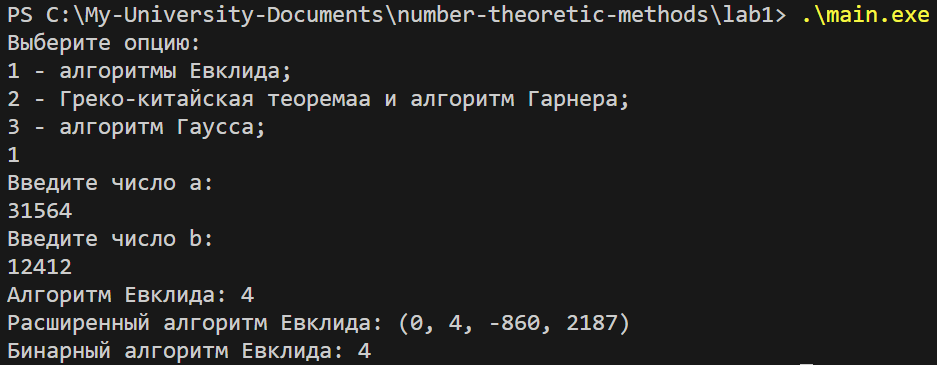
\includegraphics[width=0.8\textwidth]{pic/1.png}
            \caption{Тест алгоритмов Евклида}
        \end{figure}

        \begin{figure}[H]
            \centering
            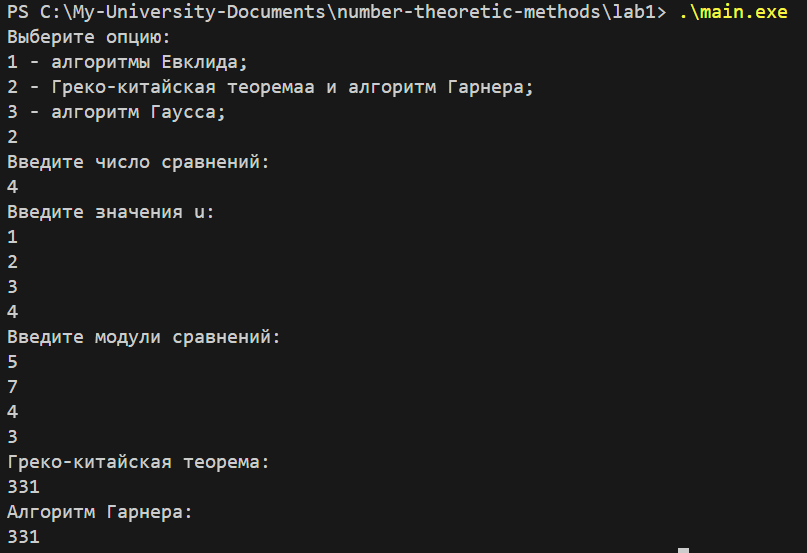
\includegraphics[width=0.8\textwidth]{pic/2.png}
            \caption{Тест алгоритмов решения систем сравнений}
        \end{figure}

        \begin{figure}[H]
            \centering
            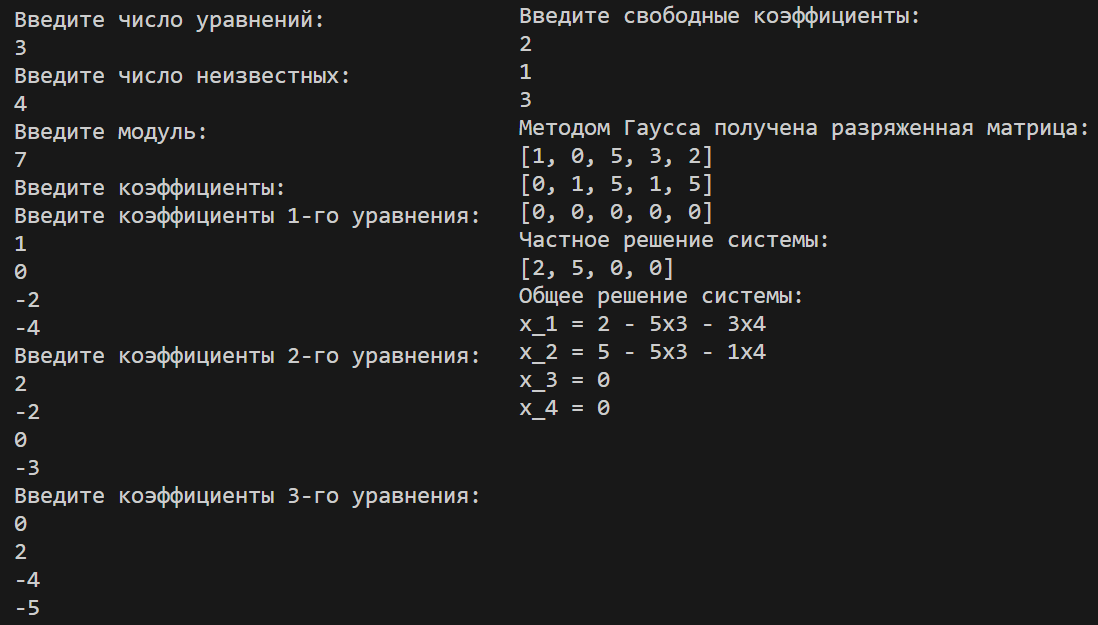
\includegraphics[width=0.8\textwidth]{pic/3.png}
            \caption{Тест реализации метода Гаусса}
        \end{figure}


\conclusion

    В данной лабораторной работе были рассмотрены теоретические сведения об
    обычном, расширенном и бинарном алгоритме Евклида, греко-китайская теорема
    об остатках, алгоритм Гарнера и метод Гаусса решения линейных уравнений над
    конечными полями. На их основе были составлены соответствующие алгоритмы.
    Была произведена оценка сложности созданных алгоритмов. Они послужили
    фундаментом для программной реализации, которая впоследствии успешно прошла
    тестирование, результаты которого были прикреплены к отчету вместе с
    листингом программы, написанной на языке Rust с использованием стандартных
    библиотек языка.

\end{document}
